\subsection{Combined data}\label{EDA}

This is a general representation of data. It combines different items from flamingo data together into one.
\begin{center}
\begin{longtable}{ |l|l| } 
 \hline
 Attribute & Description\\ 
 \hline
 userId & id of the user\\ 
 \hline
 userSessionId & id of the session\\ 
 \hline
 teamLevel & level team is at\\ 
 \hline
 platformType & what platform user is on\\ 
 \hline
 count\_gameclicks & number of game clicks\\ 
 \hline
 count\_hits & number of hits\\ 
 \hline
 count\_buyId & id of buy\\ 
 \hline
 avg\_price & average buy price\\ 
 \hline

\caption{combined-data.csv}
\end{longtable}
\end{center}

Discovering missing data showcases two things; missing data in count\_buyId and avg\_price and correlation between them. It seems like attributes are coupled together since user who buys a product gets buy ID and average price of it. Based on that logic, if item is not bought there is no ID and no price. Situation like this could be avoided by having product with id 0 and price 0 inside. This would help us expose actual missing values since at the moment we cannot confirm if missing values are intentional or by mistake.

\begin{figure}[H]
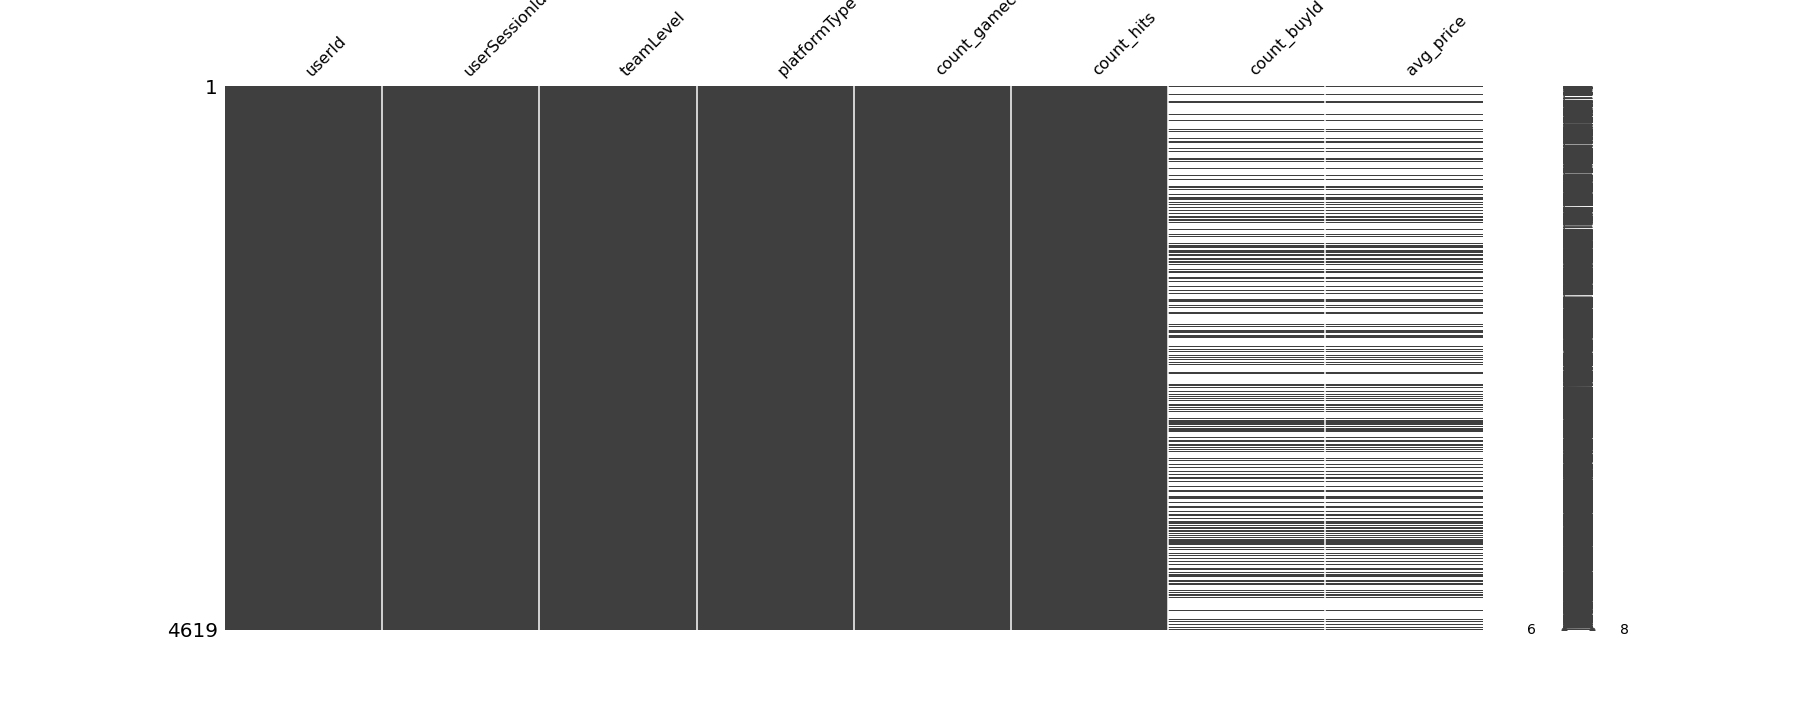
\includegraphics[scale=0.25]{img/Graphs/combinedData/missingno_combinedData.png}
\centering
\caption{combinedData\_msno}
\label{fig:combinedData_msno}
\end{figure}


Knowing our audience is key thing, therefore we need to know what platform is the most used for the game. Pie chart bellow showcases that mobile platform (mainly iphone) is what majority of our players use.
\begin{figure}[H]
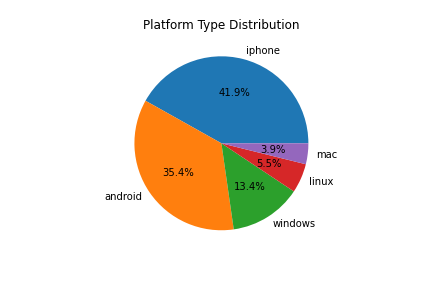
\includegraphics[scale=0.85]{img/Graphs/combinedData/correlationPlot_combinedData.png}
\centering
\caption{combinedData\_correlationPlot}
\label{fig:combinedData_correlationPlot}
\end{figure}

To understand skills, we can compare platforms between each other. Although iphone has the most game clicks (due to being the most popular) and the most hits, android seems to be fairly close to iphone. That could suggest that android players are getting more hits either due to skill or due to platform advantage.
\begin{figure}[H]
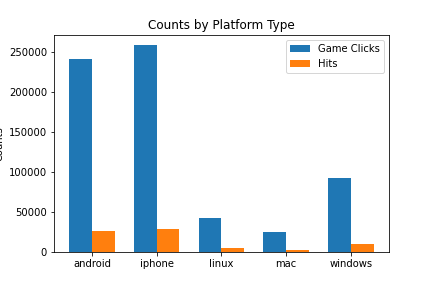
\includegraphics[scale=0.85]{img/Graphs/combinedData/multiGrap_combinedData.png}
\centering
\caption{combinedData\_multiGrap}
\label{fig:combinedData_multiGrap}
\end{figure}

Spending habits can tell us a lot about the user. By averaging price spent per platform we can see that iphone users spend the most, but what is surprising is mac users. They are second biggest spenders despite being the smallest platform (only 3.9\%). This could lead us to promote more expensive things to mac users.
\begin{figure}[H]
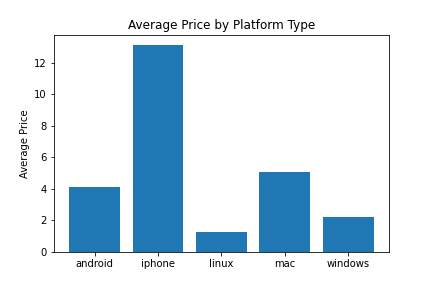
\includegraphics[scale=0.85]{img/Graphs/combinedData/priceHistogram_combinedData.png}
\centering
\caption{combinedData\_priceHistogram}
\label{fig:combinedData_priceHistogram}
\end{figure}
